%!TEX root = main.tex
\chapter{Peaceful Banana Application}
\label{peacefulBananaApplication}
In this chapter we will introduce the PeacefulBanana tool, which is the prototype we developed to support this thesis. The focus will be to explain the concept of the tool and the features and functionality it provides. The tool will be presented at a high-level, and the process of how we developed the prototype, design choices and implementation in further described in Chapter \ref{chap:design} \& \ref{chap:implementation}.
\section{What is PeacefulBanana?}
Peaceful Banana is a tool aimed towards aiding reflection in software development teams. It integrates with version control systems(VCS), which is widely used in software development. The PeacefulBanana tool collects project artifacts from such version control systems and scaffolds these in order to trigger and promote reflection in teams. PeacefulBanana will integrate with VCS and provide a layer of features specific for aiding reflection in software development projects. This means that PeacefulBanana will not feature the same functionalities that already exists in these systems, but rather contextualize them and present the data in a manner that can help teams reflect on their experiences. The tool will collect different data relevant for reflection, for example prompting the user for their mood each day, which allows for both team-wide and personal mood graphs over a period of time. \\
PeacefulBanana is developed as a web-application and will work in all modern web-browsers, on platforms like the PC, smartphones and tablets.
The tool was developed with project artifacts collected from VCS in mind. The PeacefulBanana tool will be evaluated with software development teams that have adopted an agile process model. Most agile process models feature reflection sessions in some form, in which this tool is used in order to promote and enhance reflection that takes place in these sessions. Although it is aimed at agile teams, any process model featuring some kind of reflection session could benefit from using this tool. Similarly the tool can also be used individually at any time. 

\section{What does it do?}
PeacefulBanana is a tool that allows users to reflect upon and share their experiences in development projects. The tool integrates with a VCS and focuses on collecting project artifacts like code commits, milestones, issues as well as comments and references. The tool will scaffold these data and present them to the users, acting as input for triggering reflection. The reflection will then be captured and stored as reflection notes so the user can review these at a later date. They can also be shared and used in team reflection sessions. The tool is designed to support both individual and collaborative reflection. It can be used during the team reflection workshop or just browsed individually when the user wishes to. The tool provides several opportunities to the users:
\begin{description}
	\item[Provide a scaffolded overview of the project] \hfill \\
	PeacefulBanana provides users and teams with an overview of the project:
	\begin{itemize}
		\item Users can choose what team-project to retrieve data from, see the projects milestones, issues and generate data relevant for reflection from these.
		\item The team can see when an issue has been closed, and what milestones they are connected to.
		\item The team can see which milestones were closed and when, and easily see if the team met their deadlines. 
		\item The team can see which team members have contributed to which issues.
	\end{itemize}

	\item[Individual 5-minute daily reflection] \hfill \\
	Each day a notification will prompt the user to perform a daily 5-minute reflection. This daily reflection note presents the user with data for the last 24 hours, like project activity and a tag cloud. This data provides the user with additional information and tries to trigger reflection in the users based on that day's experiences The reflection note collects input from the user:
	\begin{itemize}
		\item The user's mood that particular day, ranging 5 steps from 0 (Very sad) to 100 (Very happy)
		\item The top 2 contributions done by the user in the project that day.
		\item The top 2 fields the user can improve on in the project.
	\end{itemize}
	The PeacefulBanana application stores each of these daily summaries in a secure database. Each reflection note can also be shared with the user's team, but sharing of notes is not required. The mood data from each day is used to generate a team-wide mood-average graph, which can be used as reflection and discussion triggers in the team reflection sessions.

	\item[Reflection sessions] \hfill \\
	The team, or the team leader can create a workshop from a selected time-period. The workshop presents some mandatory questions
	related to team work and reflection. Additionally the team can choose a set of tags to generate questions from. Quick summaries of project statistics, trending issues, tag clouds and more.The finished workshop template can be printed and
	handed out to the team at the workshop, providing project statistics, trending issues, tag clouds and questions that act as reflection triggers\\
	Examples of such questions: 
		\begin{itemize}
			\item What were your initial expectations to this iteration? Did these expectations change during the iteration? How? Why?
			\item What could be done to improve team collaboration?
			\item Talk about any disappointments or successes of your project. What did you learn from it?
			\item You have had a high activity working with \#framework Did you experience any particular problems with this tag? Why or why not?
			\item What did you learn from working with the issue \textit{daily summary \& reflection notes (\#17)}?
			\item The team didn't meet the deadline for milestone \#20 - Midterm Report, did the team experience any particular problems?
		\end{itemize}
\end{description}

\section{Main goal}
The goal of the prototype is to present software development teams with a tool that can help them collect, revisit and reflect upon their experiences in both an individual and collaborative setting. Through the process of developing the prototype, it has become a tool that also supports collection of project artifacts and the presentation of these to users, in order to promote and trigger reflection. 

\section{Functionality}
% Think it would be wise to show with screenshots the different functionality (the tabs f.ex)
Reflection directed functionality:
\begin{itemize}
\item Collecting data - How a user can retrieve data and annotate it. 
\item Sharing data - How users can work together in groups to collaborate with data. 
\item Reflection triggers - Functionality developed specifically for helping users reflect on their work.
\end{itemize}

\subsection{Reflection triggers}
\paragraph{Scaffolded notes}\mbox{}\\
The tool should provide the ability to take notes in a scaffolded way, in order to avoid too generic notes. The tool will provide this functionality through collecting daily reflection notes. These notes will have questions connected to them, which triggers user to reflect on their experiences that day. Scaffolding notes this way, will prompt users to actually think about their day instead of just writing down something not useful. \\
Figure \ref{dailynote} shows an example of the PeacefulBanana reflection note. 
\begin{figure}[H]
    \centering
        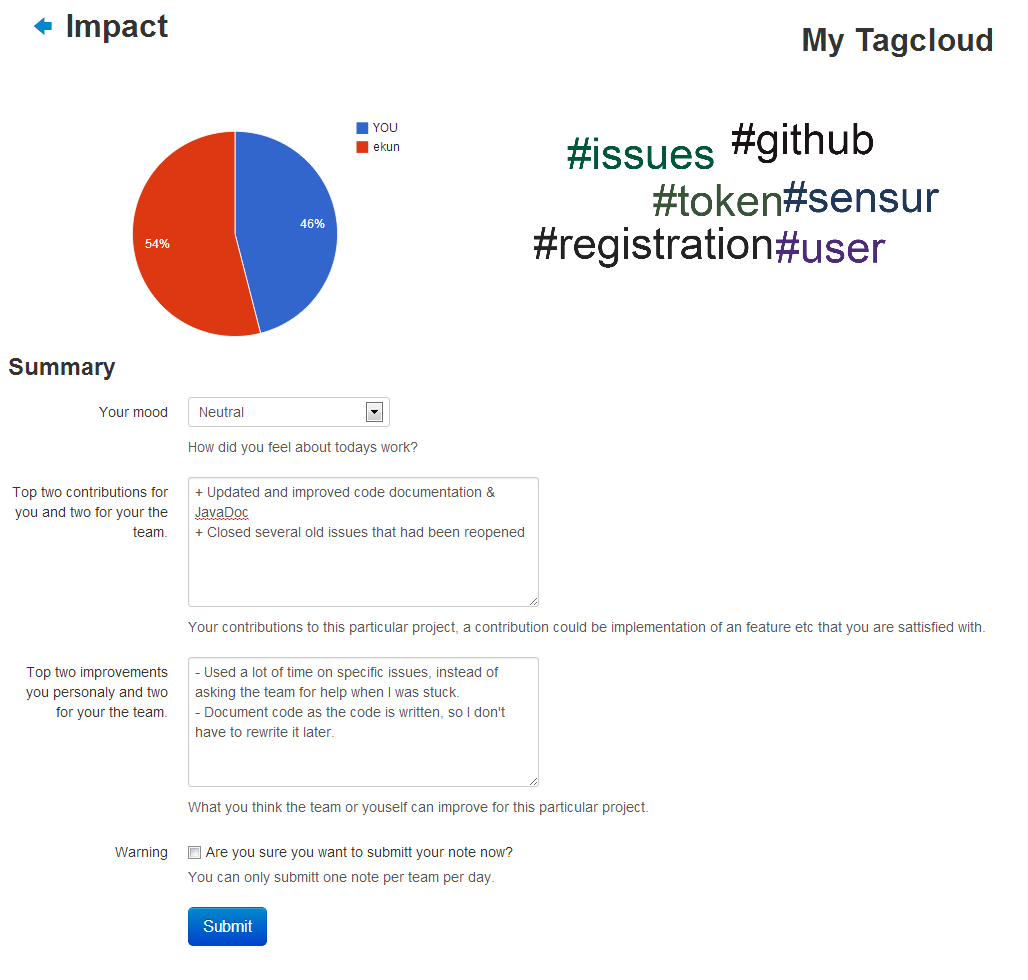
\includegraphics[width=\textwidth]{dailynote}
    \caption{PeacefulBanana reflection note}
    \label{dailynote}
\end{figure}
\paragraph{Tagclouds}\mbox{}\\
The tool should provide the ability to create tag clouds based on data divided in time. So that you can see trending events, this will enable the user to see how their work is affecting the teams work overall. These tag clouds will also give the team an indication on what the worked with over a period of time, and tags will be given a weight to show which of them that has been worked with the most. These weights will determine the words size in the tag cloud. 
\paragraph{Sharing of data}\mbox{}\\
Reflection notes can be shared with a user's team should they want to. The tool collect team-relevant data from a VCS , scaffolds and presents these to users. This data gives the team the ability to see who is working on what, are there any trending issues in the team that can be intercepted and solved and more.  
\paragraph{Mood graphs}\mbox{}\\
A user can connect his mood to reflection notes. The tool retrieves this mood data daily, in order for the tool to present meaningful mood-averages back to the users. 
The tool allows for presenting this shared team-average mood, giving an indication of how the work is perceived by the other group members and create a discussion around certain trends in mood, or even why certain users stand out from the rest of the team's mood. 
